



\section{Architecture of simulation framework} \label{sec:architecture_of_simulation_framework}


The simulation framework described in this section encompasses already described components in Section \ref{sec:r_java_simulation_framework} but enhances the framework by the cloud simulator. The cloud simulator should be able to assess the outcome of different scenarios encompassing data provided by the application server and utilizing forecast models generated on the application server in a previous step. 

The goal was to deliver a complete framework that can handle multiple data sources and is extendable for future work with possibly different data sets and an optional connection to a real cloud environment which could replace the simulated cloud environment that is connected to the framework in this implementation. 

The implementation consists of three parts which will be presented separately below. 

\paragraph{Data management} The first part represents the data handling and management interfaces presented in part already in Section \ref{sec:r_java_simulation_framework}. The purpose of this platform is to have a generic means of parsing and fetching data from various sources that can be defined in advance. For example, data may be fetched from local files that were previously retrieved from energy markets or remote web services that provide energy data of that respective energy market. In addition parsers for different file formats may be defined to automatically parse data and put it into the database for later retrieval. From there arbitrary queries may be executed to retrieve and aggregate data in a specific fashion and execute further tasks based on that data (e.g.~model generation). 

\paragraph{Forecast generation}
The second part consists of a collection of statistical methods that should assist in making accurate forecasts based on the previously collected data. A large scale evaluation of forecast methods has been presented in Section \ref{sec:forecast_model_evaluation} to determine the best forecast models for data from various energy markets. 
The purpose behind these statistical examinations is to provide meaningful and accurate forecasting models that can be utilized by the simulation framework. Eventually the performance of forecasts within the simulation should be examined and compared with approaches based solely on currently available data. It is expected that the application of accurate forecasts to energy price time series within the simulation improves overall performance and thus leads to a reduction in total energy costs. 

\paragraph{Cloud simulation}
The third part constitutes the actual cloud simulation which is based on a previously existing and sophisticated cloud simulator written in Python that incorporates cost models for energy and cooling expenses and is easily extendable by integrating custom schedulers \cite{lucanin2015philharmonic}. In this work custom settings have been applied to allow for a simulation that meets the needs of the framework to integrate different scenarios. Various parts of the simulator needed to be extended and a completely new scheduler has been built to schedule both cost aware and non-cost aware scenarios. It works together well with other parts of the framework s.t.~data can be retrieved from interfaces of the application server and integrated into the cloud simulation. The components are decoupled such that each of them may be replaced by other components easily provided that the same interface is used. 


\subsection{Architectural outline}

The architectural outline provides an overview of all components involved in the presented simulation framework and how they work together. All components may interact with one another via defined interfaces s.t.~either component may be replaced by a similar component with possibly different implementation details but same interfaces. 

\begin{figure}[htbp]
	\centering
	\vspace{-0.4in}
		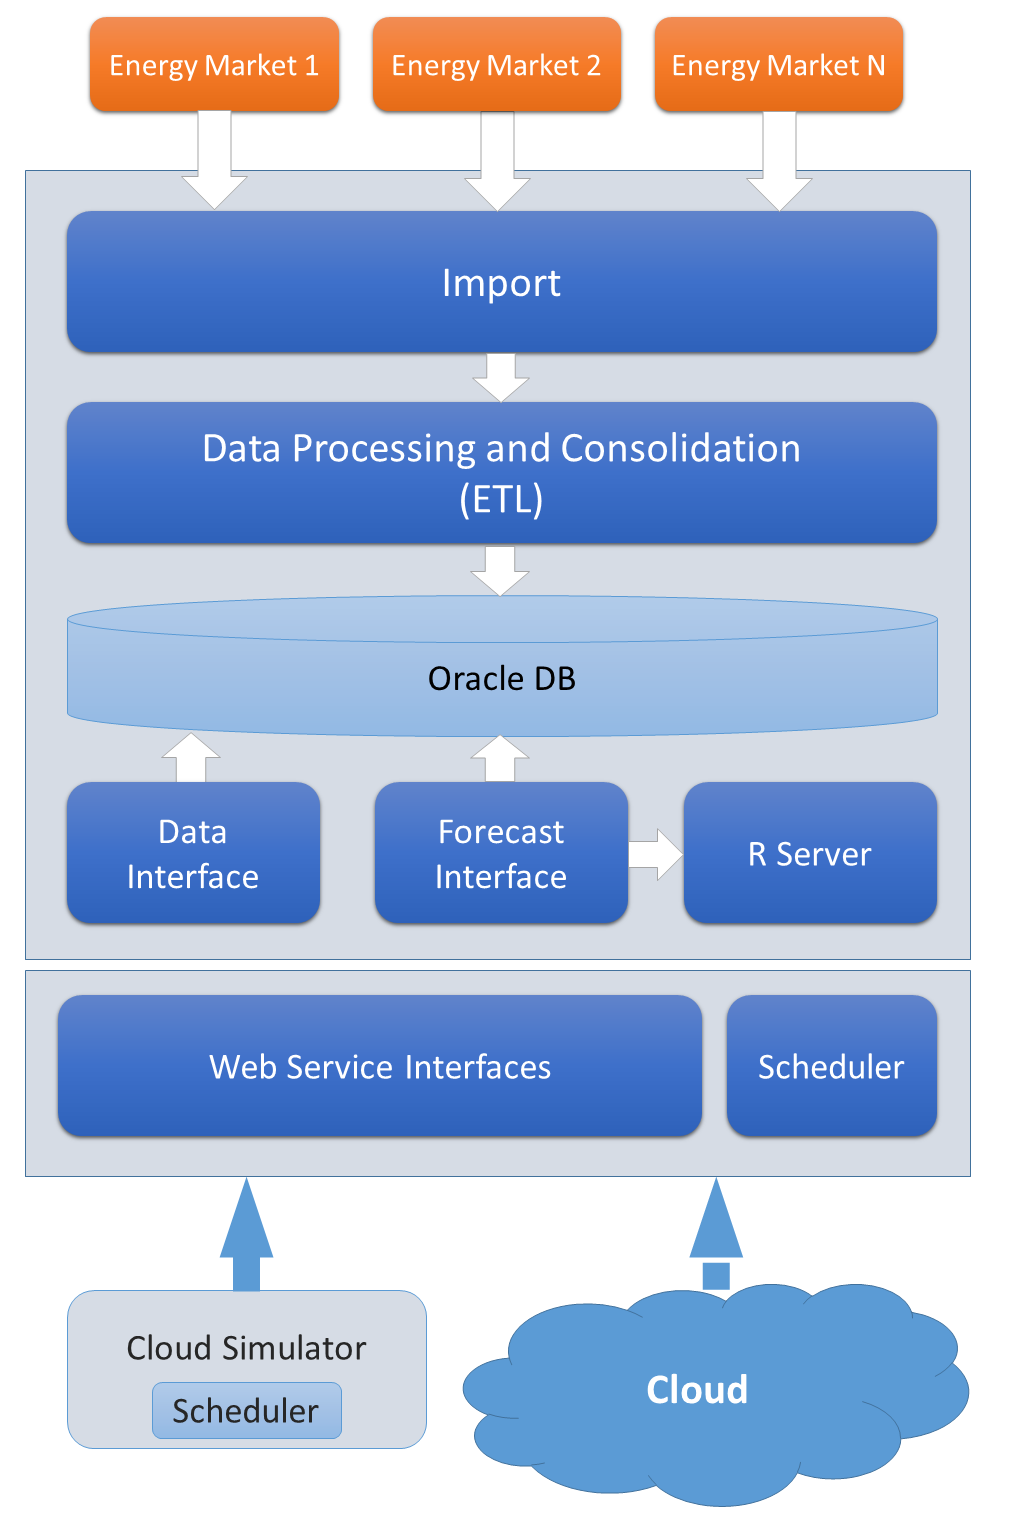
\includegraphics[width=0.5\textwidth]{figures/simulation_framework/Block_Diagram_Architecture.png}
	\caption{Architecture Block Diagram}
	\label{fig:Block_Diagram_Architecture}
\end{figure}

Figure \ref{fig:Block_Diagram_Architecture} depicts a block diagram of the simulation framework that shows which components are included and how they interact with one another. Data retrieval from the energy markets is done by the \textit{Import} module as the first action in the process. Several energy markets and their interfaces may be registered beforehand to retrieve data from these interfaces. 

From the \textit{Import} module the retrieved data is handed over to the \textit{Data Processing and Consolidation} module which transforms the data to a common format such that it can be fed to the database. This process is similar to the well known ETL process (Extract Transform Load)\cite{vassiliadis2002conceptual} which extracts data from various sources, transforms it into a defined data format and loads it into a data warehouse or database. The applied process in this work is similar as parsers for different file formats may be defined that can be configured to parse data from different sources. After the data transformation process the retrieved energy prices are stored in the database from where they may be retrieved for simulation purposes. 

The \textit{Data Interface} contains all methods for data retrieval of prices stored in the database. Thus data is provided to web service interfaces for arbitrary time periods and both day ahead and real time prices. In addition it is possible to query for local or DST corrected bidding dates or retrieving data adjusted to a predefined currency (e.g.~dollars). 

The \textit{Forecast Interface} handles all requests related to model generation and forecasting which is provided by the \textit{R server}. It contains methods defined for large scale forecast evaluation, automated model generation and calculating forecasts for generated models. 

The \textit{R server} does not directly connect to the database but retrieves energy data from the \textit{Forecast Interface} which triggers the generation of forecasting models. The interface used to communicate from Java to R (and vice versa) is called \textit{rJava} \cite{rforge2007rjava} which provides a wrapper to directly execute R code in Java. 

The \textit{Scheduler} may be configured to trigger data import from specific energy markets at a defined time interval (e.g.~every hour or once per day). In this process it may also trigger the generation of forecasting models as the model generation process can take a considerable amount of time depending on the amount of training data provided to the model.

Finally the \textit{Web Service Interfaces} are a means of providing data to external components such as the simulator or a real cloud. 
These interfaces provide data retrieval and forecast interfaces as described previously. They can be used to get historical data from different energy markets and locations as well as time periods for the purpose of getting customized data for simulations. In addition they provide a convenient way of retrieving forecast data for specific locations and periods of time. As soon as forecasting models have been generated for a specific period of time forecasts can be provided instantly for that period. 



\subsection{Components and Interfaces}

In this section a more detailed view on the various components of the framework is provided and the interfaces that exist between them. Figure \ref{fig:Component_Diagram} shows this view in form of a component diagram. 

\begin{figure}[htbp]
	% used to position the image at the horizontal center of the page
	\hspace*{-0.8in}
		% include the graphic rotated by a 90 degree angle and scale to paperwidth and height
		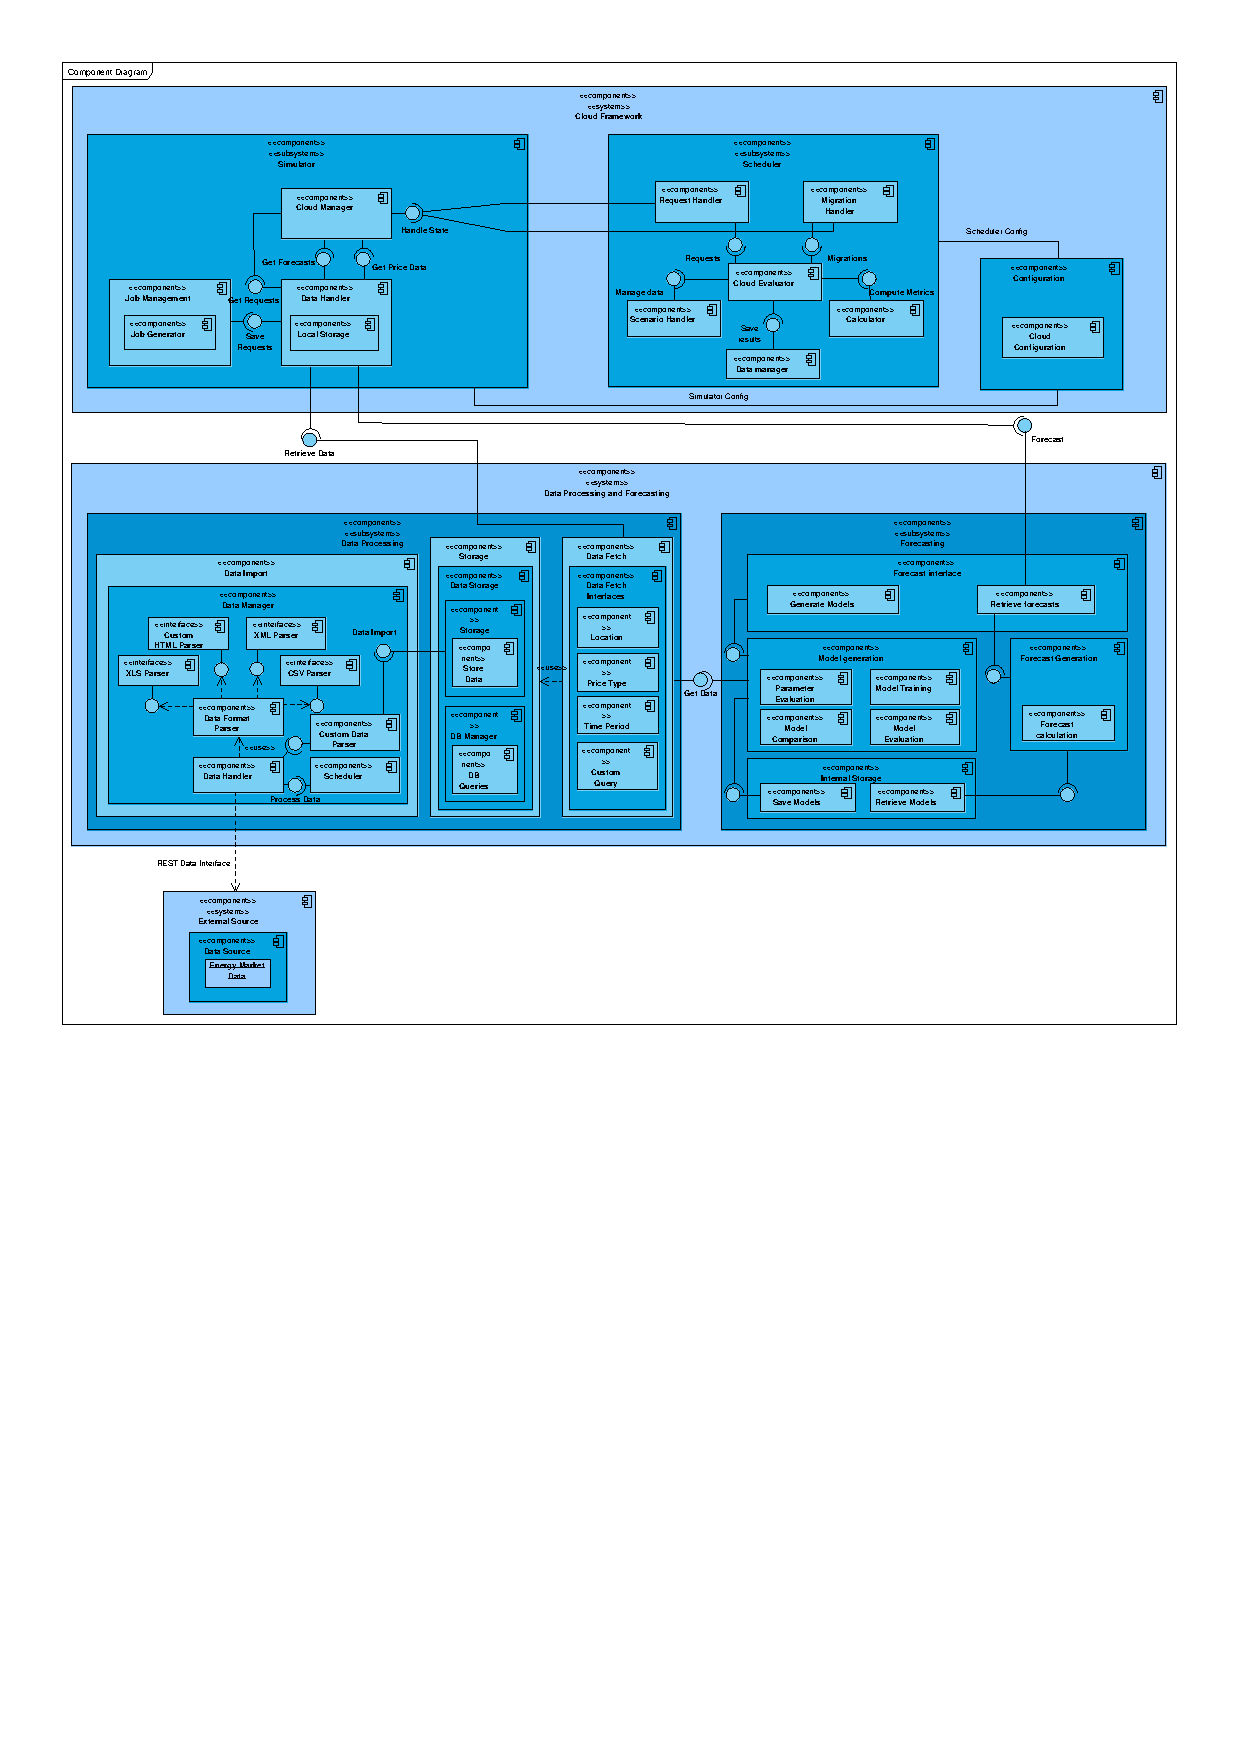
\includegraphics[angle=90,width=\paperheight,height=\paperwidth,keepaspectratio=true]{figures/simulation_framework/Component_Diagram.pdf}
	\caption{Component Diagram}
	\label{fig:Component_Diagram}
\end{figure}

The diagram basically consists of two parts, the \textit{Cloud Framework} and \textit{Data Processing and Forecasting} components. The Cloud Framework contains the \textit{Simulator} and \textit{Scheduler} and is implemented in python \cite{lucanin2015philharmonic}. It is responsible for the actual simulation and application of scheduling algorithms. The Data Processing and Forecasting part consists of the \textit{Data Processing} and \textit{Forecasting} components and is implemented on the Java application server. This component is responsible for data management and forecast operations.

\textit{Data Processing} consists of \textit{Data Import}, \textit{Storage} and \textit{Data Fetch} components. 

The \textit{Data Import} component is responsible to retrieve data from previously registered energy markets as indicated by the dashed line connection to the external data source. The data import can as well be triggered by the scheduler which calls the respective services at the Data Handler. The Data Handler uses appropriate parsers to extract data into a common processable format. When the processing of data is finished the 
data is fed to a \textit{Custom Data Parser} which handles peculiarities such as DST time changes and missing energy price data. The cleared data is then handed on to the Storage component which saves the data to the database. 

The \textit{DB Manager} in the Storage component provides methods for data retrieval which is used by the \textit{Data Fetch} component. 
Different interfaces are provided for executing queries of stored energy price data, e.g.~by location, price type or custom queries. This can in turn be used by the simulator to retrieve energy price data. 

The \textit{Forecasting} component provides interfaces to \textit{Generate Models} and \textit{Retrieve Forecasts}. 

The \textit{Generate Models} component refers to the \textit{Model Generation} component with \textit{Parameter Evaluation}, \textit{Model Training}, \textit{Model Evaluation} and \textit{Model Comparison}. Before model generation it refers to the Data Fetch component for retrieval of energy price data of the desired time period. After the model(s) have been generated they are saved to the \textit{Internal Storage}, i.e.~in the file system of the application server. 

For retrieving forecasts the \textit{Retrieve Forecasts} interface is queried which in turn calls the \textit{Forecast Generation} component. Thus forecasts may be retrieved from models which have been generated and stored previously within the Internal Storage component. 

fetches data from the database and does some data preprocessing that is used for forecasting. After the data has been processed and formatted appropriately it is ready to be analyzed by statistical methods to determine which forecasting model suits best for the selected time series. Different models are trained and compared and the best model is chosen. It is then selected by the Forecast Module and the actual forecasts are calculated which can be queried via a provided public interface that is exposed to external systems. 

The \textit{Cloud Framework} uses the historical price data provided by the \textit{Data Fetch} component to run simulations for various scenarios. It is read into a local storage by a \textit{Data Handler} for further processing of the price data in simulations. In addition, forecasts may be retrieved by the Data Handler at this stage to prevent having an open connection to the application server during simulations. Job requests are generated by the \textit{Job Management} component which reflect certain characteristics or requirements of tasks that should be processed by the Cloud Framework. Requests and energy prices are read by the \textit{Cloud Manager} that keeps track of the cloud's current state. The state is retrieved and modified by the scheduler which retrieves data from \textit{Request} and \textit{Migration Handlers} which is then fed to the \textit{Cloud Evaluator}. The evaluator decides on needs for migrations depending on the given scenario defined by the \textit{Scenario Handler}. It uses a \textit{Calculator} component to compute metrics such as migration energy and VM downtime. 

At each step the Cloud Evaluator gets current request and migration demands and checks metrics for VM migration. If it retrieves a positive result the resources are moved to the respective server. Results are handled by a Data Manager component after the simulation finishes. Both scheduler and simulator components are configurable by a config file defined by the \textit{Cloud Configuration} component. Thus new configuration options are easily added and can be changed at any time to adjust the output of simulations. 




\section{Modeling migration energy}

Besides the structural outline presented in the previous section important methodologies used by the cloud simulator and scheduler are investigated in detail in the following sections. 

Since the goal of the simulation presented in this work is to reduce energy costs by intelligently migrating resources across geo-distributed data centers an important metric to consider is the migration energy and migration costs. An outstanding paper on this topic has been presented in \cite{liu2013performance} where the energy and downtime related to a VM migration are examined and formalized in detail. This paper has been briefly outlined in Section \ref{ssec:performance_and_energy_modeling_of_virtual_machines}. 

The impact of the \textit{writable working set} (WWS) of an application on VM migration time and total downtime is described in \cite{clark2005live} (see also Section \ref{ssec:live_migration_of_virtual_machines}). It is the set of most frequently updated memory pages in a running application which is dirtied in each pre-copy round of an VM migration \cite{clark2005live, liu2013performance}. Thus a large WWS can increase migration downtime significantly with a high amount of pages dirtied in each pre-copy iteration (dirty page rate) that ultimately have to be sent at a time at the final stop-and-copy phase. 

With increasing number of iterations more data has to be transferred and transmission costs rise. The final stop-and-copy phase is reached when any of the following conditions has been met (as implemented in this work): 

\begin{enumerate}[label=\textnormal{(\arabic*)}]
	\item memory dirtying rate exceeds memory transmission rate \label{itm:condition1}
	\item the remaining dirty memory falls below a predefined threshold \label{itm:condition2}
	\item the number of pre-copying iterations exceeds a defined maximum \label{itm:condition3}
\end{enumerate}

From \cite{liu2013performance} the proposed base model for VM migration has been implemented. It is based on a list of parameters defined in Table \ref{tab:migration_parameters}. 

Migration energy, load and downtime metrics have been implemented based on the following equations: 

\begin{align}
	\lambda &= \frac{D}{R} \label{eq:m_lambda} \\
	V_i &= D \frac{V_{mem}}{R} \lambda^{i-1} = V_{mem} \lambda^i \label{eq:m_v_i} \\
	T_i &= \frac{D T_{i-1}}{R} = \frac{V_{mem} D^i}{R^{i+1}} = \frac{V_{mem} \lambda^i}{R} \label{eq:m_t_i} \\
	V_{mig} &= \sum_{i=0}^n V_i = V_{mem} \frac{1 - \lambda^{n+1}}{1 - \lambda} \label{eq:m_v_mig} \\
	T_{mig} &= \sum_{i=0}^n T_i = \frac{V_{mem}}{R} \frac{1 - \lambda^{n+1}}{1 - \lambda} \label{eq:m_t_mig} \\
	n &= \left\lceil \log_{\lambda} \frac{V_{thd}}{V_{mem}} \right\rceil \label{eq:m_n} \\
	T_{down} &= T_n + T_{resume} \label{eq:m_t_down} \\
	E_{mig} &= E_{sour} + E_{dest} \label{eq:m_e_mig} \\
	&= (\alpha_s + \alpha_d) V_{mig} + (\beta_s + \beta_d) \nonumber \\
	&= \alpha V_{mig} + \beta \nonumber \\
	V_n \le V_{thd} &\Leftrightarrow V_{mem} \lambda^n \le V_{thd} \label{eq:m_v_n}
\end{align}


\begin{table}[htbp]
\centering
\begin{tabular}{ll}
  \hline
	Parameter & Description \\ 
  \hline
		$V_{mem}$ & The total size of the VM memory \\ 
		$V_{mig}$ & The total migration load (network traffic) during migration \\ 
		$T_{mig}$ & Total migration time \\ 
		$V_i$ & Migration load for the i-th iteration \\ 
		$T_i$ & Migration transfer time for the i-th iteration \\ 
		$T_{down}$ & Effective downtime of migration \\ 
		$T_{resume}$ & Time to resume operation of VM on other host \\ 
		$E_{mig}$ & Total migration energy \\ 
		$\alpha, \beta$ & Model parameters for migration energy \\
		$R$ & Memory transmission rate or bandwidth \\ 
		$D$ & Dirty page rate of application \\ 
		$V_{thd}$ & Threshold of remaining memory to end pre-copy phase \\ 
		$\lambda$ & Convergence coefficient of VM migration \\ 
		$n$ & The index of the last pre-copy iteration \\
		$n_{max}$ & The maximum number of pre-copy iterations \\
   \hline
\end{tabular}
\caption{Parameters used in the migration algorithm}
\label{tab:migration_parameters}
\end{table}


Equation \ref{eq:m_lambda} defines $\lambda$ as the convergence coefficient of the migration since it states how fast the migration converges to the final stop-and-copy phase. 

$V_i$ and $T_i$ in Equations \ref{eq:m_v_i} and \ref{eq:m_t_i} denote the migration load and time in iteration $i$ where these metrics depend greatly on the convergence coefficient $\lambda$. If $D < R$ then $\lambda < 1$ and migration load will eventually fall below the defined threshold $V_{thd}$ (assuming a writable working set less than $V_{thd}$). 

$V_{mig}$ and $T_{mig}$ in Equations \ref{eq:m_v_mig} and \ref{eq:m_t_mig} describe the total migration load and time which is defined as the sum of migration load and time for all iterations $i$ up to the last iteration $n$. Equation \ref{eq:m_n} defines the index of the last pre-copy iteration after which the stop-and-copy phase is executed. 

Equation \ref{eq:m_t_down} describes the effective downtime of the migration consisting of the time needed for the last iteration (stop-and-copy phase) and the time needed to resume operation of the newly created VM. Equation \ref{eq:m_e_mig} formalizes migration energy as the sum of source and destination energy ($E_{sour}$ and $E_{dest}$). Model parameters $\alpha$ and $\beta$ can each be defined separately for source and destination (e.g.~$\alpha_s$ and $\alpha_d$). However in this work homogenous parameters have been assumed for both source and destination (last line of the equation). 

The condition for reaching the defined memory threshold is depicted in Equation \ref{eq:m_v_n}. As defined before $n$ is the index of the last pre-copy iteration where remaining memory should be below threshold $V_{thd}$ (see definition of condition \ref{itm:condition2}). In case this condition is not met and $n = n_{max}$ the pre-copy phase is aborted and all remaining memory is transferred to the destination host (condition \ref{itm:condition3}). When condition \ref{itm:condition1} is detected data is transferred at once. 



\section{Cost optimization based on utility function}


